\documentclass[12pt]{ctexart}
\usepackage{geometry}       % 设置页面整体布局
\geometry{top=2.5cm, bottom=2.5cm, left=2cm, right=2cm}
\usepackage{fancyhdr}       % 设置页眉页脚布局
\pagestyle{fancy}
\rhead{\thepage}            % 设置右页眉为页数
\chead{中国科学技术大学}
\cfoot{}                    % 设置中间页脚为空
\usepackage{amsmath}        % 数学公式宏包
\numberwithin{equation}{section}
\usepackage{esint}          % 交叉引用宏包
\usepackage[colorlinks,     % 设置引用的颜色
            linkcolor=black,
            anchorcolor=black,
            urlcolor=cyan,
            citecolor=black,
           ]{hyperref}
\usepackage{makecell}       % 插入表格宏包
\usepackage{longtable}      % 长表格宏包
\usepackage{appendix}       % 生成附录宏包
\usepackage{graphicx}       % 插入图片宏包
\usepackage{epstopdf}       % 插入eps图片宏包
\usepackage{cite}           % 文献引用宏包
\renewcommand{\thefigure}   % 设置图片编号格式
    {\thesection{}.\arabic{figure}}
\renewcommand{\thefootnote}{} % 设置角标编号不出现在文中
                            % 以\footnotetext{Footnotetext without footnote mark}使用
\usepackage{unicode-math}
\usepackage{listings}
\usepackage{hyperref}



\CTEXsetup[format={\Large\bfseries}]{section}


\begin{document}

\nocite{*}

\begin{center}
    \heiti \fontsize{24pt}{0}{乙酸乙酯皂化反应动力学研究}

    \vspace{12pt}

    \kaishu \fontsize{13.75pt}{0}禤科材

    \footnotetext{\textbf{实验日期:}2022年10月14日}
    \footnotetext{\textbf{作者简介:}禤科材(2002-),男,学号PB20030874,中国科学技术大学本科在读,专业方向为化学物理}
    \footnotetext{\textbf{联系方式:}电话 18108064415 ,邮箱 \href{mailto:ustcxkc@mail.ustc.edu.cn}{ustcxkc@mail.ustc.edu.cn}}

    \vspace{5pt}

    \songti \fontsize{12pt}{0}(中国科学技术大学化学与材料科学学院,安徽 合肥 230026)
\end{center}

\noindent\textbf{摘~~~\!要}~~~\!
乙酸乙酯的皂化反应是一个二级反应。若起始物浓度相同,则二级反应为
纯二级反应。由于体系的电导率与产物中CH$_3$COO$^−$的浓度具有明确
关系且易于测量,本次实验采用测定电导率的方式获得乙酸乙酯水解过程中
浓度与时间变化的关系,并以此获得该反应的速率常数。由于实验数据严重偏离物理实际,活化能通过查阅资料给出。报告同时
进行了总结讨论,指出了现有电导法测定速率常数的不足之处,并提供了
可行的改进建议。
\newline
\textbf{关键字}~~~\!
二级反应;电导率;速率常数;活化能

\begin{center}
    {\LARGE\rmfamily\textbf{The Kinetic Study on Saponification of Ethyl Acetate}}

    \vspace{12pt}

    {\slshape Xuan Kecai}

    \vspace{5pt}

    (School of Chemistry and Material Science, USTC, Hefei 230026, China)
\end{center}

\noindent\textbf{Abstract}~~~\!
The saponification of ethyl acetate is a second-order
reaction. If the concentration of the starting material is
the same, the second-order reaction is a pure second-order
reaction. Because the conductivity of the system has a clear
relationship with the concentration of CH$_3$COO$^−$ in the
product and is easy to measure, the relationship between the
concentration and time during the hydrolysis of ethyl
acetate is obtained by measuring the conductivity, and the
rate constants of the reaction are
obtained.Since the experimental data deviated from the physical reality seriously, the activation energy was from the references. At the same time, the report summarizes and
discusses, points out the shortcomings of the existing
conductivity method for determining the rate constant, and
provides feasible suggestions for improvement.
\newline
\textbf{Keywords}~~~\!
second order reaction; conductivity; reaction rate constant;
activation energy

\section{序言}

乙酸乙酯是应用最广的脂肪酸酯之一,是重要的化工原料,在制药工业和
有机合成上发挥着重要作用。乙酸乙酯容易水解,常温下有水存在时,
也逐渐水解生成乙酸和乙醇。添加微量的酸或碱能促进水解反应。乙酸乙酯
的碱性水解与酸性水解最大的差别在于碱性水解是不可逆的。乙酸与乙醇
发生可逆反应会生成乙酸乙酯。陈酒味道比新酒香,就是因为酒中少量的
乙酸与乙醇反应生成具有果香味的乙酸乙酯。

皂化反应通常指的是碱(通常为强碱)和酯反应,而生产出醇和羧酸盐,
尤指油脂和碱反应。狭义的讲,皂化反应仅限于油脂与氢氧化钠或氢氧化钾
混合,得到高级脂肪酸的钠/钾盐和甘油的反应。这个反应是制造肥皂流程
中的一步,因此而得名。它的化学反应机制于 1823 年被法国科学家
Eug\'ene Chevreul 发现。皂化反应除常见的油脂与氢氧化钠反应外,还有
油脂与浓氨水的反应。

皂化反应在洗涤用品的工业合成等方面十分常见。因此,对皂化反应的
动力学研究具有重要的理论意义和实用价值。

\section{实验}
\subsection{实验原理}

在碱性条件下,乙酸乙酯可以发生皂化反应,水解成醋酸和乙醇
\begin{align}
    \mathrm{CH_3COOCH_2CH_3 + OH^- \longrightarrow CH_3COO^- + CH_3CH_2OH}.
\end{align}

这是一个二级反应。当反应物的初始浓度均为$a$时,该反应为纯二级反应。
设$t$时刻各生成物的浓度均为$x$,则有积分式
\begin{align}
    kt = \frac{x}{a(a-x)}.
\end{align}

在反应的过程中,不同时刻各物种的浓度难以直接测量,故通过测量溶液的
电导率来反应浓度的变化。电导仪采用交流电极,交流频率很快,其发生的
电极反应无法持续进行,不会对反应体系物质浓度造成影响。对于电流密度
不太大的一般液体体系,溶液中的电流主要由正负离子的运动承担。由于
$\mathrm{CH_3COO^−}$的迁移率比$\mathrm{OH^−}$小,反应过程中体系的
电导率值会不断下降。在一定范围内,体系电导率的减少量和
$\mathrm{CH_3COO^−}$浓度的增加量成正比,则体系电导率与时间具有
明确的关系
\begin{align}
    \frac{L_0 - L_t}{t} = akL_t - akL_\infty.
\end{align}

其中,$L_0$、$L_t$、$L_\infty$ 分别是初始时刻、$t$时刻、反应完全
进行时的电导率。做$(L_0 - L_t)/t \sim L_t$图像,通过斜率就可以
计算出反应速率常数,再通过截距可以得到反应完全进行时的电导率。测量
两个温度下的速率常数,通过 Arrhenius 公式就可以得到反应的活化能
$^{[1]}$。

\subsection{试剂与仪器}

乙酸乙酯(国药集团化学试剂有限公司,AR)、NaOH(片状,国药集团化学
试剂有限公司,AR)、邻苯二甲酸氢钾(国药集团化学试剂有限公司,AR)、
酚酞(国药集团化学试剂有限公司,AR)。

SevenMulti 型pH/电导率/离子综合测试仪(Mettler Toledo 国际有限
公司)、HK-2A 型超级恒温水水浴(南京南大万和科技有限公司)、
CPA2245 型分析天平(Sartorius)、JB-1B 型磁力搅拌器(上海雷磁
新泾仪器有限公司)、100 mL 移液管、100$\mu$L 移液枪、100 mL 恒温
夹套反应器、50 mL 滴定管、250 mL 锥形瓶、1000 mL 广口瓶、50 mL
烧杯、洗耳球。

\subsection{实验方法}
\subsubsection{NaOH 浓度的标定}

称量大约2 g NaOH 并加入约100 mL 蒸馏水配制成浓 NaOH 溶液。
在1000 mL 广口瓶中装入约900 mL 蒸溜水,在搅拌下逐滴加入浓 NaOH
溶液并测量电导率至 1300$\sim$1400 $\mu$S/cm。将配制好的 NaOH
溶液用邻苯二甲酸氢钾和酚酞在室温下滴定,重复三次以上,计算出 NaOH
的准确浓度和后续实验需要的乙酸乙酯体积。

\subsubsection{\texorpdfstring{$L_0$的测定}{L0 的测定}}

精确移取 100 mL 滴定好的 NaOH 溶液于30$^\circ$C 恒温夹套反应器中,
插入洗净且吸干水的测量电极,恒温10分钟,当电导仪上的读数稳定后,
每隔1 min 读取一次数据,测定三个平行的数据。

\subsubsection{\texorpdfstring{$L_t$的测定}{Lt 的测定}}

使用移液枪所需用量的乙酸乙酯,穿过大口玻璃套,全部放入溶液中,不要
遗留在玻璃套的内壁上,以免浓度不准。立即打开电导率仪读数,每隔10 s
读一次数,持续35分钟。

将温度改为35$^\circ$C,重复2.3.1节和2.3.2节的实验步骤。

\section{结果与讨论}
\subsection{实验结果}
\subsubsection{NaOH 浓度的标定}

由滴定数据可以算出,NaOH 的浓度为 5.42$\times 10^{-3}$ mol/L,
故每组实验应注入的乙酸乙酯体积为51 $\mu$L。

\subsubsection{\texorpdfstring{30$^\circ$C 下的实验结果}{30 度下的实验结果}}

在30.0$^\circ$C 的条件下,测得 NaOH 的电导率为 1446 $\mu$S/cm。
注入51 $\mu$L 乙酸乙酯后记录数据,可见数据点并不完全分布在一条直线上。以线性相关系数大于等于 $0.999$ 为标准选择数据,用 Mathematica 拟合得到$(L_0 - L_t)/t \sim L_t$图像
如图3.1所示。
\begin{figure}[!h]
    \centering
    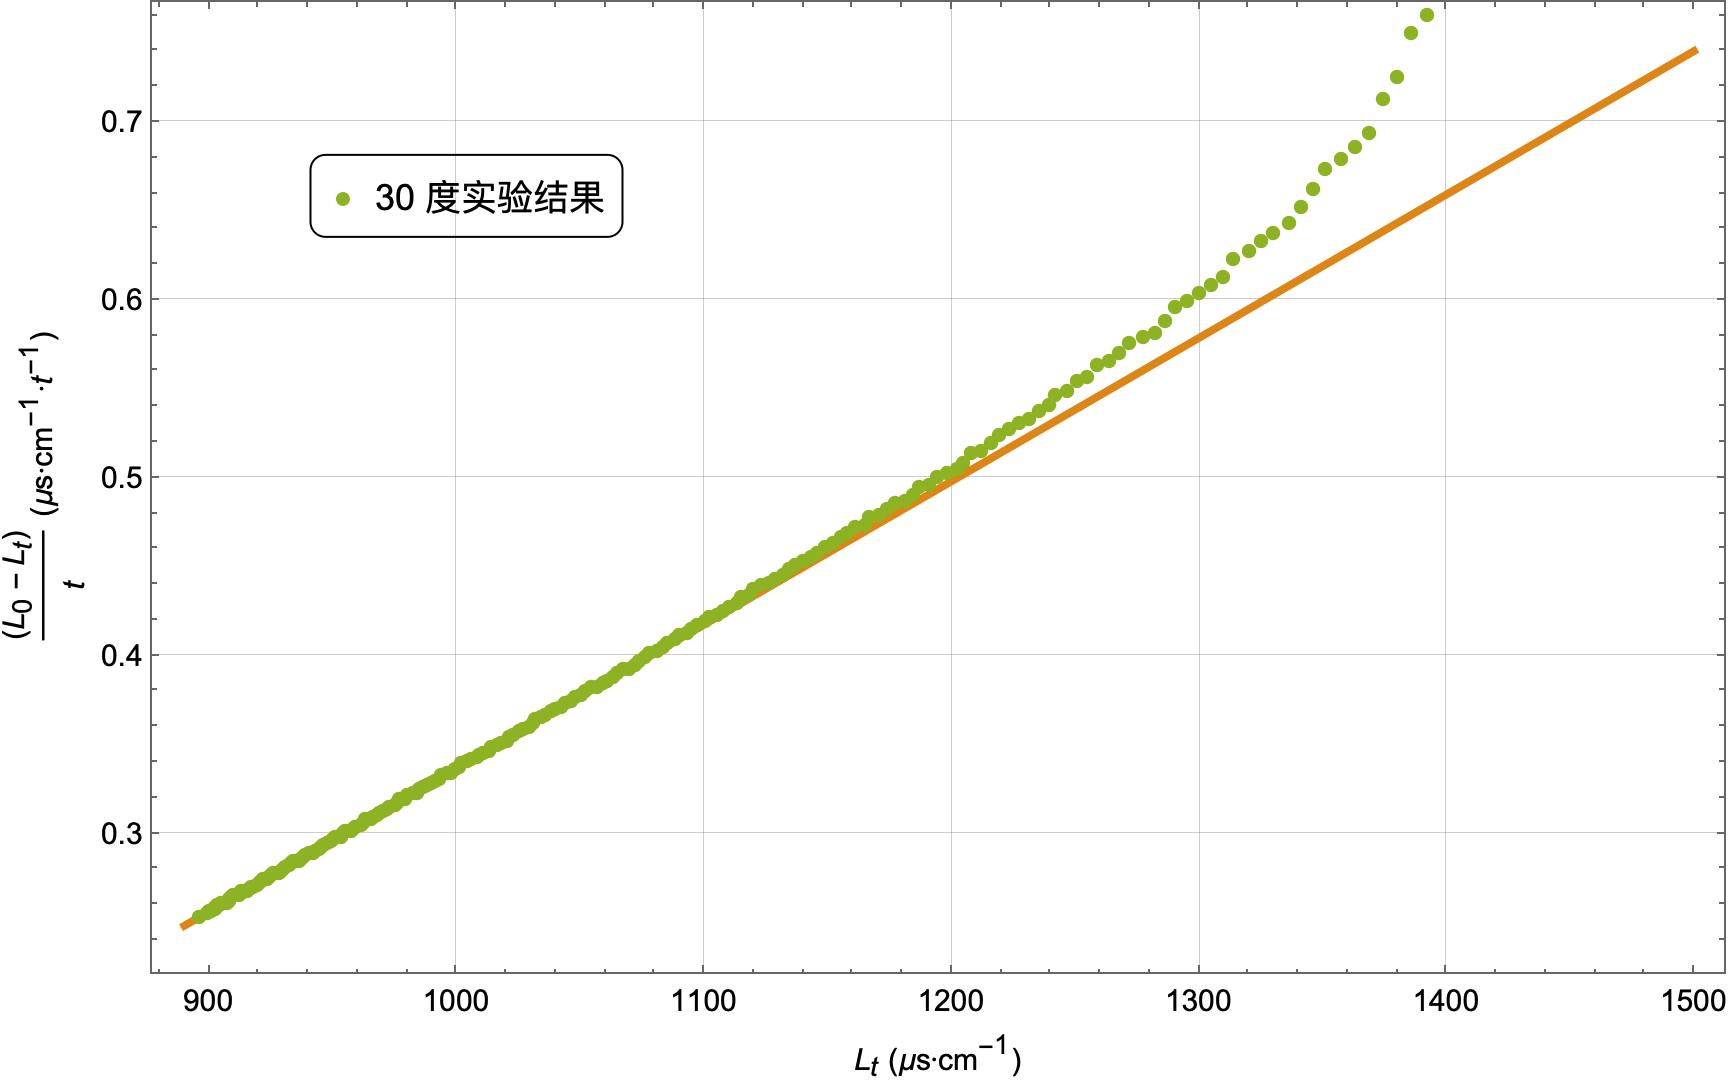
\includegraphics[scale=0.45]{30degree.jpg}
    \caption{30$^\circ$C 下的拟合图像}
\end{figure}

相应的拟合直线方程为
\begin{align}
    (L_0 - L_t)/t = 8.06 \times 10^{-4} L_t - 0.469.
\end{align}

线性相关系数 $R^2 = 0.99974$,反应速率常数为$k = $0.14 mol/(L$\cdot$s),反应完全进行后的
电导率为$L_\infty = $581 $\mu$S/cm。

\subsubsection{\texorpdfstring{35$^\circ$C 下的实验结果}{35 度下的实验结果}}

在34.9$^\circ$C 的条件下,测得 NaOH 的电导率为1591 $\mu$S/cm。
注入51 $\mu$L 乙酸乙酯后记录数据。数据点并不完全分布在一条直线上。以线性相关系数大于等于 $0.999$ 为标准选择数据,用 Mathematica 拟合得到$(L_0 - L_t)/t \sim L_t$图像
如图3.2所示。
\begin{figure}[!h]
    \centering
    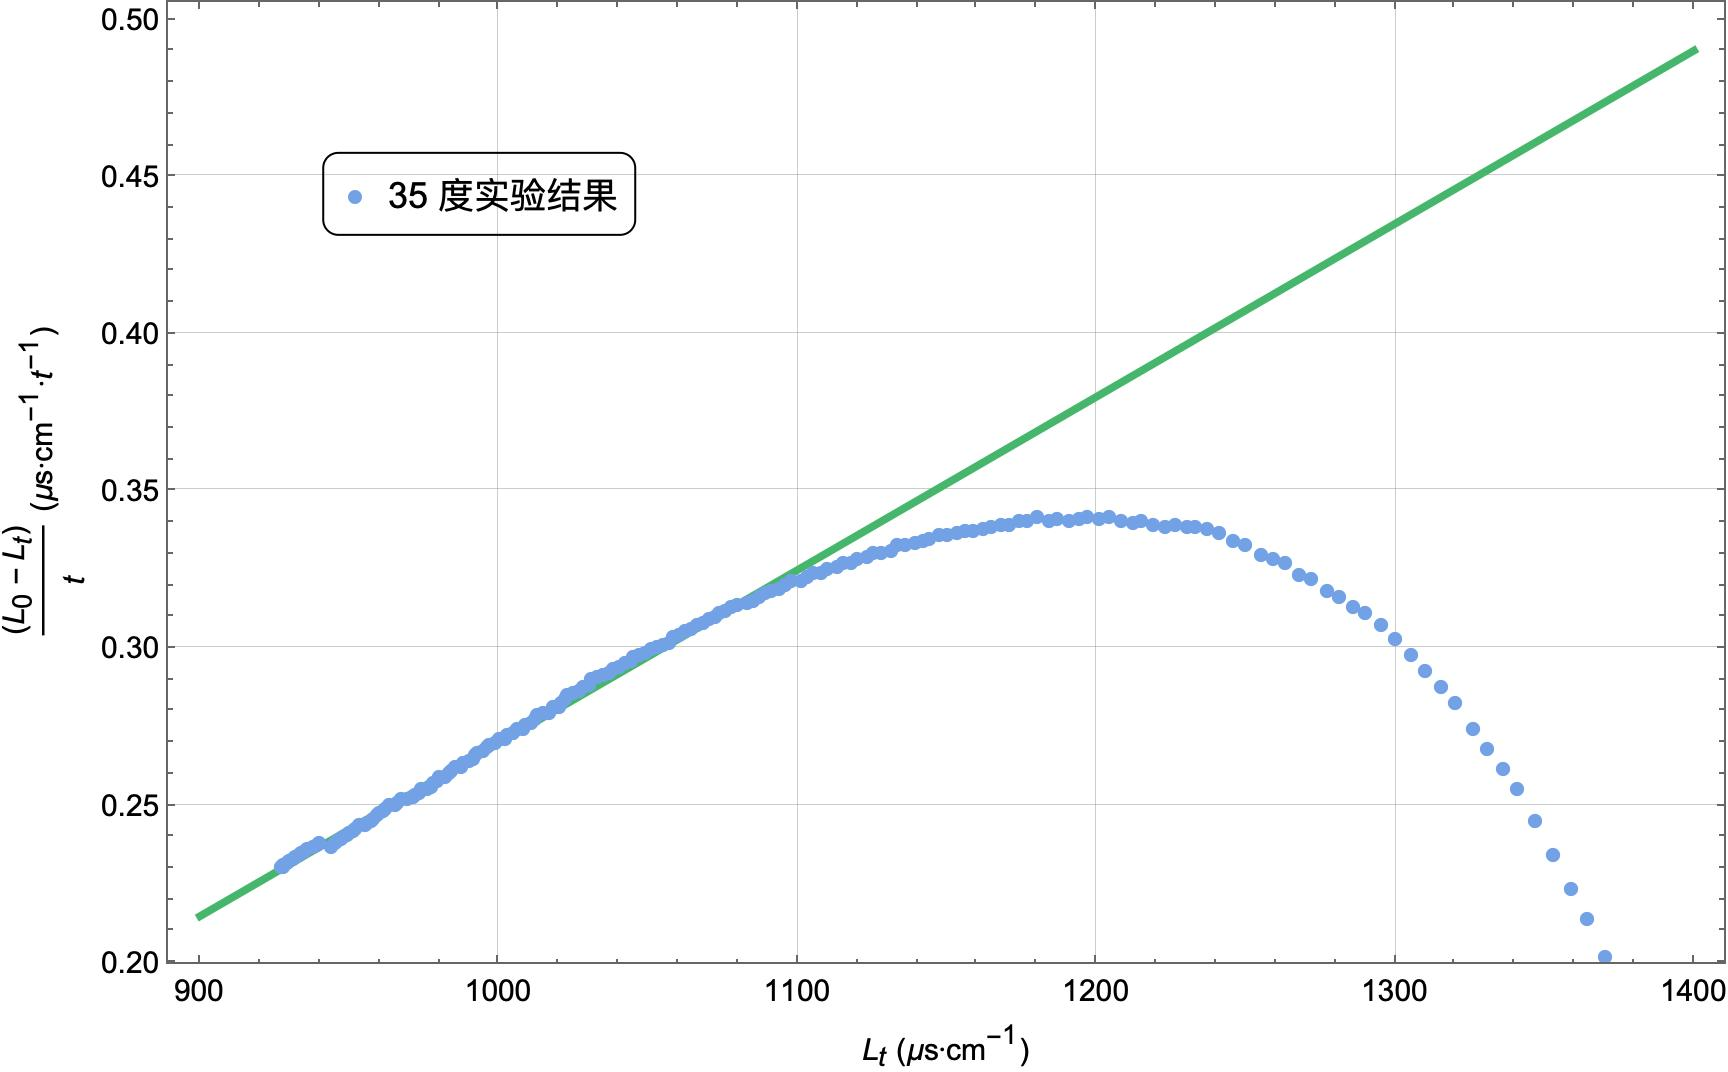
\includegraphics[scale=0.45]{35degree.jpg}
    \caption{35$^\circ$C 下的拟合图像}
\end{figure}

相应的拟合直线方程为
\begin{align}
    (L_0 - L_t)/t = 5.50 \times 10^{-4} L_t - 0.280.
\end{align}

线性相关系数 $R^2 = 0.999675$,反应速率常数为$k = $0.10 mol/(L$\cdot$s),反应完全进行后的
电导率为$L_\infty = $703 $\mu$S/cm。

\subsubsection{\texorpdfstring{反应的活化能$E_a$}{反应的活化能}}

由实验数据可以看出,在本实验中,30度计算得到的反应速率常数大于35度计算得到的反应速率常数,如果直接带入Arrhenius 公式,将会得到负的活化能,不符合物理实际。所以不作计算,应当分析实验失败的原因。

查阅资料可知,胡获华和尹力$^{[3]}$用相同方法测得的活化能为45.10 kJ/mol。

\subsection{误差分析}
\subsubsection{系统误差}

(1)本实验最明显的误差在于35度下的反应速率常数竟然低于30度下的反应速率常数,这是因为在操作过程中升温时间较长,恒温箱内的温度总是在34.2-34.5之间徘徊。这直接导致了导致准确标定、准确移取的 NaOH 溶液在较高温度的条件下与空气接触时间过长,进而发生显著的消耗。这不仅影响了溶液的电导率,还使得溶液PH值降低、与乙酸乙酯进行的反应速率减慢,从而发生了实验中的偏差。

(2)实验原理中假设醋酸钠完全电离。但实际上,由于醋酸是弱酸,醋酸根
会发生少量的水解。由于水解现象的存在,电导率与反应进行程度并不是
严格的线性关系,因此会对实验结果造成一定的影响。

(3)实验中假设起始物浓度相同,将反应化为纯二级反应。但在操作上
该条件由于移液枪精度的限制难以精确实现。因此实验得到的曲线会略向
混二级反应偏离,造成一定的误差。

(4)活化能的大小与温度有关。实验采用 Arrhenius 公式计算活化能,
忽略的温度的影响,而实际过程中反应温度会在小幅度范围内变化,因此
会给实验结果造成一定的误差。

(5)观察数据文件可知,仪器在计时时并非每次都是准确的间隔10 s 进行
读数,有少量11 s 的情况存在。故平均的读数时间间隔略大于10 s。但在
进行数据处理时,默认数据的读数间隔的准确的10 s,这会带来一定的误差。

\subsubsection{偶然误差}

(1)实验中 NaOH 溶液在存放过程中会吸收空气中的二氧化碳,使氢氧根
离子浓度降低,且生成的碳酸根离子也会对溶液的电导率造成一定的影响。

(2)实验采用滴定的方式测定 NaOH 溶液的浓度。由于氢氧化钠溶液浓度
极稀,因而滴定过程很容易受到空气中二氧化碳的干扰;且由于氢氧根
离子浓度低,酚酞的变色也较浅,终点难以准确判断,靠人眼辨别误差较大。

(3)滴定过程中,部分组别的滴定实验起始时并未将滴定管液面调至
0.00 mL 处。由分析化学实验所学知识可知,滴定管在20$\sim$30 mL
处的示数最为准确。两次连续滴定并未调整液面至0.00 mL,这将使得最终
滴定完成时液面处在50 mL 附近,此处的读数精准度略低,造成实验误差
增大。

(4)实验中在每个温度下都只进行了一次测量,存在数据偶然性。应多次
测量取平均值以减小偶然误差。同时,实验数据处理仅使用两个不同温度下
的数据计算反应活化能,误差较大。应当在一系列不同温度下进行实验,用
速率常数对温度做线性拟合,以求出反应活化能。

\subsection{实验讨论与改进方法}
\subsubsection{温度对速率常数及活化能的影响}

将两次实验的数据作在同一张图中,如图3.3所示。由该图像可以看出,随着温度的升高,反应速率常数和反应完全进行时的
电导率都会增大。这是因为,温度上升后,反应物分子的平均能量升高,
反应物分子更容易越过活化能垒而发生反应,故反应速率加快,速率常数
增大;同时,温度升高可以促进电解质的电离,反应生成的醋酸根等
弱电解质电离程度增大,故电导率增大。

\begin{figure}[!h]
    \centering
    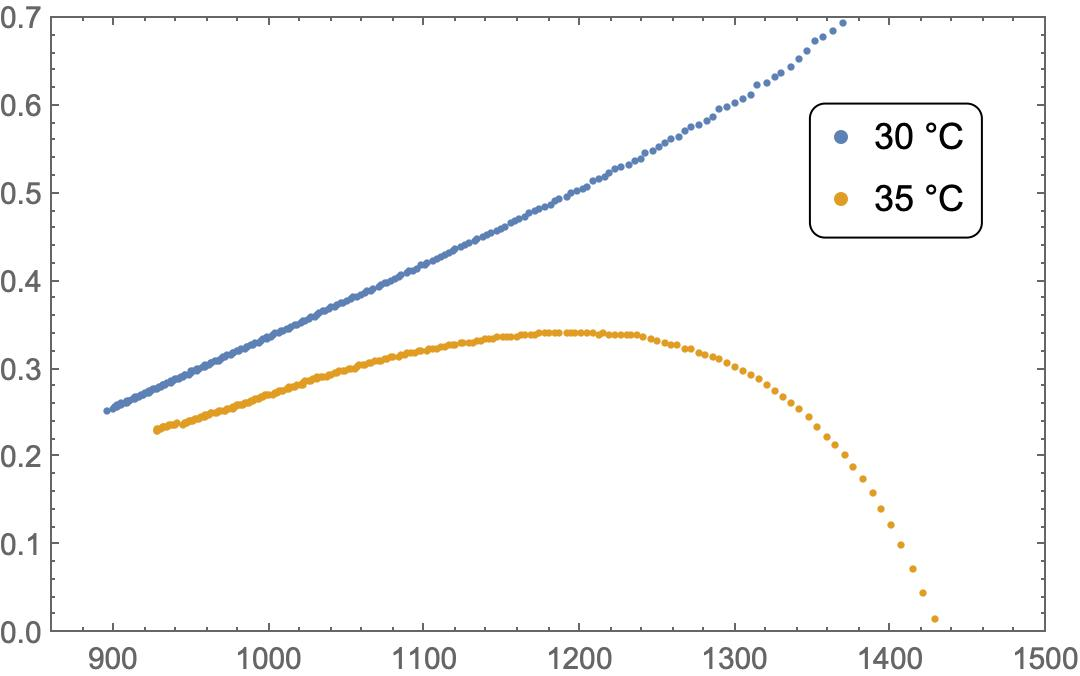
\includegraphics[scale=0.67]{inone.jpg}
    \caption{两个温度下的数据图像}
\end{figure}

\subsubsection{数据点右侧的向下偏移现象}

观察数据图像可以发现,图像右侧的数据点存在向下偏移的现象。

反应初期,体系中刚刚加入乙酸乙酯即开始计时读数。此时乙酸乙酯在反应
体系中还未分散均匀。乙酸乙酯的扩散需要时间,这相当于增大了起始阶段
的时间$t$。纵坐标中$t$位于分母,因此图像右侧的数据点向下偏移。随着
时间的推进,乙酸乙酯逐渐混合均匀,图像偏移量逐渐减小。

\subsubsection{实验方案改进}

凌锦龙等人$^{[3]}$在处理实验数据时采用了微元的方法。文献指出,作
$(tL_t − t′Lt′)/∆t \sim (L′_t − L_t)/\Delta t$图也可以得到
线性关系,而无需测量$L_0$。同时,文献的误差分析部分指出,由误差
传递公式,若将$L_0$的值改变1\%,计算出的速率常数$k$的相对误差高达
7\%。因此避免测量$L_0$对实验精度的提高具有重大意义。

\section{结语}

本实验通过测量反应稳定时电导率的方法得到乙酸乙酯皂化反应这一典型
二级反应的反应速率常数和活化能,在30.0$^\circ$C 下,反应速率常数
为0.14 mol/(L$\cdot$s),在34.9$^\circ$C 下,反应速率常数为
0.10 mol/(L$\cdot$s)。数据严重违反物理实际,经分析是由精确标定的NaOH溶液在较高温度的条件下与空气作用过久而导致的电导率下降、PH降低、反应速率减慢等一系列误差所致。

所以,本实验在温度控制方面必须严格把关,不能让NaOH在较高温度下和空气作用太长时间,同时容器的密闭程度也应当改进。
\pagebreak
\begin{center}
    \Large\bfseries{参考文献}
\end{center}
\noindent
[1] 傅献彩, 沈文霞, 姚天扬等. 物理化学(第五版). 上册[M].
高等教育出版社,2006.

\noindent
[2] 胡跃华, 尹力. 乙酸乙酯皂化反应速度常数及活化能测定的研究[J].
大学化学, 1989(05): 40-45.

\noindent
[3] 凌锦龙. 乙酸乙酯皂化反应实验数据处理方法的改进[J]. 通化师范
学院学报, 2005, 026(002): 49-5.

\newpage

\begin{center}
    \LARGE\bfseries{附录~~~实验数据处理}
\end{center}
\begin{center}
    \Large\bfseries{附录I~~~实验数据处理}
\end{center}

\subsection*{I.1~~~NaOH 浓度的标定}

实验数据如下表所示。

\begin{longtable}{|c|c|c|c|c|}
    \caption{NaOH 浓度标定数据} \\
    \hline
    组别 & 1 & 2 & 3 & 4\\
    \hline
    $m$(KHP)/g & 0.0300 & 0.0254 & 0.0292 & 0.0277 \\
    \hline
    $V$(NaOH)/mL & 26.50 & 22.90 & 26.35 & 25.00 \\
    \hline
    $c$(NaOH)/($\times 10^{-3}$mol/L) & 5.54 & 5.43 & 5.42 & 5.42 \\
    \hline
    $c$(NaOH)/($\times 10^{-3}$mol/L) & / & \multicolumn{3}{c|}{5.42} \\
    \hline
    相对偏差/\% & / & 0.18\% & 0\% & 0\% \\
    \hline
\end{longtable}

第一组实验误差较大,故舍去。由2、3、4组实验数据计算得到,氢氧化钠
溶液浓度为5.42$\times 10^{-3}$mol/L,实验相对偏差均在0.2\%以内,数据有效。

\subsection*{I.1~~~ $L_t$的测定和$k$的计算}

由实验数据可以读出,系统稳定在30.0$^\circ$C 后,测得 NaOH 的电导率
为1446 $\mu$S/cm。注入51 $\mu$L 乙酸乙酯后记录数据,可见数据点并不完全分布在一条直线上。以线性相关系数大于等于 $0.999$ 为标准,用 Mathematica 拟合得到$(L_0 - L_t)/t \sim L_t$图像如图4.4所示。

\begin{figure}[!h]
    \centering
    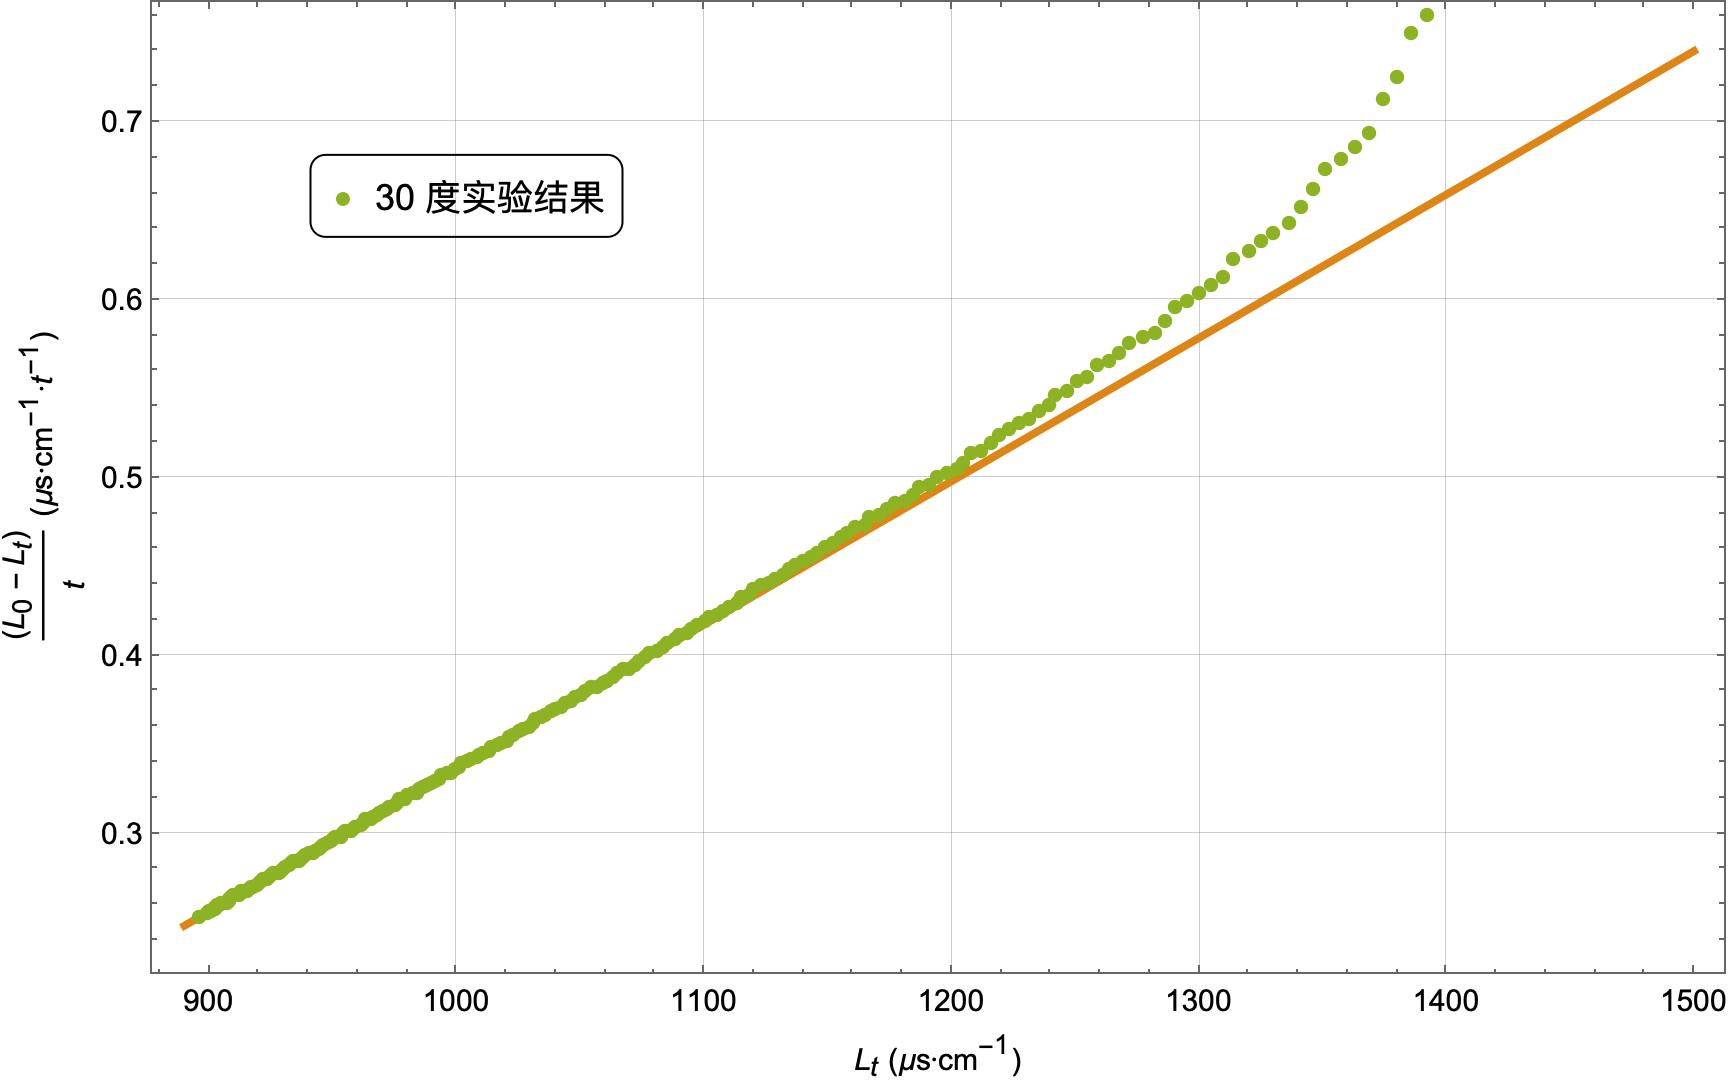
\includegraphics[scale=0.45]{30degree.jpg}
    \caption{30$^\circ$C 下的拟合图像}
\end{figure}

相应的拟合直线方程为
\begin{align}
    (L_0 - L_t)/t = 8.06 \times 10^{-4} L_t - 0.469.
    \tag{I.1}
\end{align}

由实验原理可知,拟合直线的斜率即为$ak$。其中$a$为反应物初始浓度,
$k$为反应速率常数。反应物初始浓度均为5.42$\times$10$^{-3}$
mol/L,故可得反应速率常数为$k = $0.14 mol/(L$\cdot$s)。

由实验原理可知,拟合直线的截距即为$-akL_\infty$。故可得反应完全
进行后的电导率为$L_\infty$ = 581 $\mu$S/cm。

由实验数据可以读出,系统稳定在34.9$^\circ$C 后,测得 NaOH 的电导率
为1591 $\mu$S/cm。注入51 $\mu$L 乙酸乙酯后,以线性相关系数大于等于 $0.999$ 为标准选取500s后的数据。用 Mathematica 拟合得到
$(L_0 - L_t)/t \sim L_t$图像如图4.5所示。
\begin{figure}[!h]
    \centering
    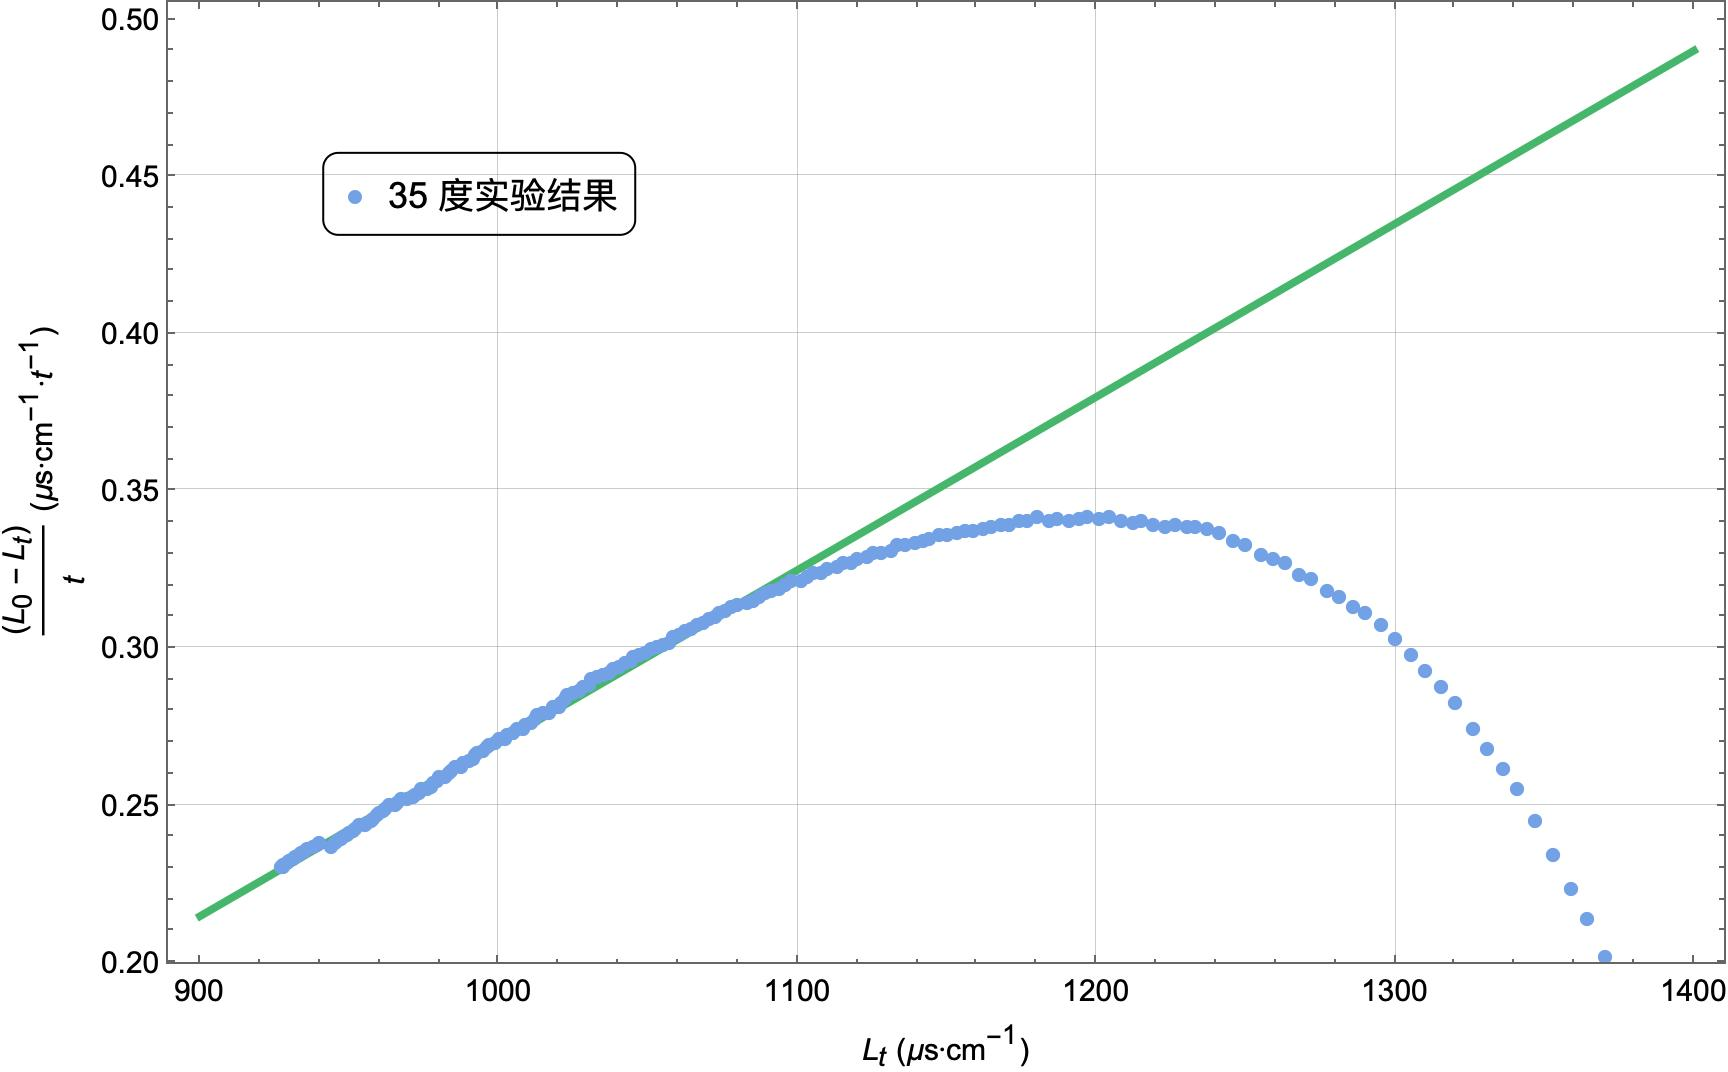
\includegraphics[scale=0.45]{35degree.jpg}
    \caption{35$^\circ$C 下的拟合图像}
\end{figure}

相应的拟合直线方程为
\begin{align}
    (L_0 - L_t)/t = 5.50 \times 10^{-4} L_t - 0.280.
    \tag{I.2}
\end{align}

由实验原理可知,拟合直线的斜率即为$ak$。其中$a$为反应物初始浓度,
$k$为反应速率常数。反应物初始浓度均为5.42$\times$10$^{-3}$
mol/L,故可得反应速率常数为$k = $0.10 mol/(L$\cdot$s)。

由实验原理可知,拟合直线的截距即为$-akL_\infty$。故可得反应完全
进行后的电导率为$L_\infty$ = 703 $\mu$S/cm。

\subsection*{I.2~~~ 反应活化能$E_a$的计算}

由实验数据可以看出,在本实验中,30度计算得到的反应速率常数大于35度计算得到的反应速率常数,如果直接带入Arrhenius 公式,将会得到负的活化能,不符合物理实际。所以不作计算,应当分析实验失败的原因。

物理化学教材$^{[1]}$中有类似的习题,其基本计算过程如下:将29.75$^\circ$C 和35.28$^\circ$C 的实验数据带入 Arrhenius 公式
\begin{align}
    \ln\frac{k_2}{k_1} = -\frac{E_a}{R}
    \left(\frac{1}{T_2} - \frac{1}{T_1}\right)
    \tag{I.3}
\end{align}
可得
\begin{align}
    E_a
    &= -\frac{R\ln(k_2 / k_1)}{1/T_2 - 1/T_1} \notag\\
    &= -\frac{8.314 \times 10^{-3} \times \ln(0.21 / 0.16)}
        {1/(273.15+35.28) - 1/(273.15+29.75)} \tag{I.4} \\
    &= 38~\mathrm{(kJ\cdot mol^{-1})}. \notag
\end{align}

故该反应的表观活化能为$E_a = 38~\mathrm{kJ\cdot mol^{-1}}$。

\begin{center}
    \Large\bfseries{附录II~~~原始数据记录}
\end{center}

\begin{longtable}{cc|cc}
    \caption{30$^\circ$C 溶液电导率数据(每隔 10 s 记录一次)} \\
    \hline
    时间 & 电导率/$\mu s\cdot cm^{-1}$ & 时间 & 电导率/$\mu s\cdot cm^{-1}$ \\
    \hline
    Fri 14 Oct 2022 18:00:30 & 1446 & Fri 14 Oct 2022 18:18:38 & 1042 \\
Fri 14 Oct 2022 18:00:40 & 1431 & Fri 14 Oct 2022 18:18:48 & 1040 \\
Fri 14 Oct 2022 18:00:50 & 1423 & Fri 14 Oct 2022 18:18:58 & 1038 \\
Fri 14 Oct 2022 18:01:00 & 1417 & Fri 14 Oct 2022 18:19:08 & 1036 \\
Fri 14 Oct 2022 18:01:10 & 1410 & Fri 14 Oct 2022 18:19:18 & 1034 \\
Fri 14 Oct 2022 18:01:20 & 1405 & Fri 14 Oct 2022 18:19:28 & 1032 \\
Fri 14 Oct 2022 18:01:30 & 1398 & Fri 14 Oct 2022 18:19:38 & 1031 \\
Fri 14 Oct 2022 18:01:41 & 1392 & Fri 14 Oct 2022 18:19:48 & 1029 \\
Fri 14 Oct 2022 18:01:50 & 1386 & Fri 14 Oct 2022 18:19:58 & 1027 \\
Fri 14 Oct 2022 18:02:01 & 1380 & Fri 14 Oct 2022 18:20:08 & 1025 \\
Fri 14 Oct 2022 18:02:11 & 1374 & Fri 14 Oct 2022 18:20:19 & 1023 \\
Fri 14 Oct 2022 18:02:21 & 1369 & Fri 14 Oct 2022 18:20:29 & 1021 \\
Fri 14 Oct 2022 18:02:31 & 1363 & Fri 14 Oct 2022 18:20:39 & 1020 \\
Fri 14 Oct 2022 18:02:41 & 1357 & Fri 14 Oct 2022 18:20:49 & 1018 \\
Fri 14 Oct 2022 18:02:51 & 1351 & Fri 14 Oct 2022 18:20:59 & 1016 \\
Fri 14 Oct 2022 18:03:01 & 1346 & Fri 14 Oct 2022 18:21:09 & 1014 \\
Fri 14 Oct 2022 18:03:11 & 1341 & Fri 14 Oct 2022 18:21:19 & 1013 \\
Fri 14 Oct 2022 18:03:21 & 1336 & Fri 14 Oct 2022 18:21:29 & 1011 \\
Fri 14 Oct 2022 18:03:32 & 1330 & Fri 14 Oct 2022 18:21:39 & 1009 \\
Fri 14 Oct 2022 18:03:41 & 1325 & Fri 14 Oct 2022 18:21:49 & 1008 \\
Fri 14 Oct 2022 18:03:51 & 1320 & Fri 14 Oct 2022 18:21:59 & 1006 \\
Fri 14 Oct 2022 18:04:02 & 1314 & Fri 14 Oct 2022 18:22:09 & 1004 \\
Fri 14 Oct 2022 18:04:12 & 1310 & Fri 14 Oct 2022 18:22:19 & 1002 \\
Fri 14 Oct 2022 18:04:22 & 1305 & Fri 14 Oct 2022 18:22:30 & 1001 \\
Fri 14 Oct 2022 18:04:32 & 1300 & Fri 14 Oct 2022 18:22:40 & 999 \\
Fri 14 Oct 2022 18:04:42 & 1295 & Fri 14 Oct 2022 18:22:50 & 998 \\
Fri 14 Oct 2022 18:04:52 & 1290 & Fri 14 Oct 2022 18:23:00 & 996 \\
Fri 14 Oct 2022 18:05:02 & 1286 & Fri 14 Oct 2022 18:23:10 & 994 \\
Fri 14 Oct 2022 18:05:12 & 1282 & Fri 14 Oct 2022 18:23:20 & 993 \\
Fri 14 Oct 2022 18:05:22 & 1277 & Fri 14 Oct 2022 18:23:30 & 991 \\
Fri 14 Oct 2022 18:05:32 & 1272 & Fri 14 Oct 2022 18:23:40 & 990 \\
Fri 14 Oct 2022 18:05:42 & 1268 & Fri 14 Oct 2022 18:23:50 & 988 \\
Fri 14 Oct 2022 18:05:52 & 1264 & Fri 14 Oct 2022 18:24:00 & 986 \\
Fri 14 Oct 2022 18:06:02 & 1259 & Fri 14 Oct 2022 18:24:10 & 985 \\
Fri 14 Oct 2022 18:06:13 & 1255 & Fri 14 Oct 2022 18:24:20 & 984 \\
Fri 14 Oct 2022 18:06:22 & 1251 & Fri 14 Oct 2022 18:24:30 & 982 \\
Fri 14 Oct 2022 18:06:33 & 1247 & Fri 14 Oct 2022 18:24:40 & 980 \\
Fri 14 Oct 2022 18:06:43 & 1242 & Fri 14 Oct 2022 18:24:51 & 979 \\
Fri 14 Oct 2022 18:06:53 & 1239 & Fri 14 Oct 2022 18:25:01 & 977 \\
Fri 14 Oct 2022 18:07:03 & 1235 & Fri 14 Oct 2022 18:25:11 & 976 \\
Fri 14 Oct 2022 18:07:13 & 1231 & Fri 14 Oct 2022 18:25:21 & 975 \\
Fri 14 Oct 2022 18:07:23 & 1227 & Fri 14 Oct 2022 18:25:31 & 973 \\
Fri 14 Oct 2022 18:07:33 & 1223 & Fri 14 Oct 2022 18:25:41 & 972 \\
Fri 14 Oct 2022 18:07:43 & 1219 & Fri 14 Oct 2022 18:25:51 & 970 \\
Fri 14 Oct 2022 18:07:53 & 1216 & Fri 14 Oct 2022 18:26:01 & 969 \\
Fri 14 Oct 2022 18:08:04 & 1212 & Fri 14 Oct 2022 18:26:11 & 968 \\
Fri 14 Oct 2022 18:08:13 & 1208 & Fri 14 Oct 2022 18:26:21 & 966 \\
Fri 14 Oct 2022 18:08:24 & 1205 & Fri 14 Oct 2022 18:26:31 & 965 \\
Fri 14 Oct 2022 18:08:33 & 1202 & Fri 14 Oct 2022 18:26:41 & 963 \\
Fri 14 Oct 2022 18:08:44 & 1198 & Fri 14 Oct 2022 18:26:51 & 962 \\
Fri 14 Oct 2022 18:08:54 & 1194 & Fri 14 Oct 2022 18:27:01 & 961 \\
Fri 14 Oct 2022 18:09:04 & 1191 & Fri 14 Oct 2022 18:27:12 & 959 \\
Fri 14 Oct 2022 18:09:14 & 1187 & Fri 14 Oct 2022 18:27:22 & 958 \\
Fri 14 Oct 2022 18:09:24 & 1184 & Fri 14 Oct 2022 18:27:32 & 957 \\
Fri 14 Oct 2022 18:09:34 & 1181 & Fri 14 Oct 2022 18:27:42 & 955 \\
Fri 14 Oct 2022 18:09:44 & 1177 & Fri 14 Oct 2022 18:27:52 & 954 \\
Fri 14 Oct 2022 18:09:54 & 1174 & Fri 14 Oct 2022 18:28:02 & 953 \\
Fri 14 Oct 2022 18:10:04 & 1171 & Fri 14 Oct 2022 18:28:12 & 951 \\
Fri 14 Oct 2022 18:10:14 & 1167 & Fri 14 Oct 2022 18:28:22 & 950 \\
Fri 14 Oct 2022 18:10:24 & 1165 & Fri 14 Oct 2022 18:28:32 & 949 \\
Fri 14 Oct 2022 18:10:34 & 1161 & Fri 14 Oct 2022 18:28:42 & 948 \\
Fri 14 Oct 2022 18:10:45 & 1158 & Fri 14 Oct 2022 18:28:52 & 946 \\
Fri 14 Oct 2022 18:10:54 & 1155 & Fri 14 Oct 2022 18:29:02 & 945 \\
Fri 14 Oct 2022 18:11:05 & 1152 & Fri 14 Oct 2022 18:29:12 & 944 \\
Fri 14 Oct 2022 18:11:15 & 1149 & Fri 14 Oct 2022 18:29:23 & 943 \\
Fri 14 Oct 2022 18:11:25 & 1146 & Fri 14 Oct 2022 18:29:33 & 942 \\
Fri 14 Oct 2022 18:11:35 & 1143 & Fri 14 Oct 2022 18:29:43 & 940 \\
Fri 14 Oct 2022 18:11:45 & 1140 & Fri 14 Oct 2022 18:29:53 & 939 \\
Fri 14 Oct 2022 18:11:55 & 1137 & Fri 14 Oct 2022 18:30:03 & 938 \\
Fri 14 Oct 2022 18:12:05 & 1134 & Fri 14 Oct 2022 18:30:13 & 937 \\
Fri 14 Oct 2022 18:12:15 & 1132 & Fri 14 Oct 2022 18:30:23 & 936 \\
Fri 14 Oct 2022 18:12:25 & 1129 & Fri 14 Oct 2022 18:30:33 & 934 \\
Fri 14 Oct 2022 18:12:36 & 1126 & Fri 14 Oct 2022 18:30:43 & 933 \\
Fri 14 Oct 2022 18:12:45 & 1123 & Fri 14 Oct 2022 18:30:53 & 932 \\
Fri 14 Oct 2022 18:12:56 & 1120 & Fri 14 Oct 2022 18:31:03 & 931 \\
Fri 14 Oct 2022 18:13:05 & 1118 & Fri 14 Oct 2022 18:31:13 & 930 \\
Fri 14 Oct 2022 18:13:15 & 1115 & Fri 14 Oct 2022 18:31:23 & 929 \\
Fri 14 Oct 2022 18:13:26 & 1113 & Fri 14 Oct 2022 18:31:33 & 928 \\
Fri 14 Oct 2022 18:13:36 & 1110 & Fri 14 Oct 2022 18:31:44 & 926 \\
Fri 14 Oct 2022 18:13:46 & 1108 & Fri 14 Oct 2022 18:31:54 & 925 \\
Fri 14 Oct 2022 18:13:56 & 1105 & Fri 14 Oct 2022 18:32:04 & 924 \\
Fri 14 Oct 2022 18:14:06 & 1102 & Fri 14 Oct 2022 18:32:14 & 923 \\
Fri 14 Oct 2022 18:14:16 & 1100 & Fri 14 Oct 2022 18:32:24 & 922 \\
Fri 14 Oct 2022 18:14:26 & 1097 & Fri 14 Oct 2022 18:32:34 & 921 \\
Fri 14 Oct 2022 18:14:36 & 1095 & Fri 14 Oct 2022 18:32:44 & 920 \\
Fri 14 Oct 2022 18:14:46 & 1093 & Fri 14 Oct 2022 18:32:54 & 919 \\
Fri 14 Oct 2022 18:14:56 & 1090 & Fri 14 Oct 2022 18:33:04 & 918 \\
Fri 14 Oct 2022 18:15:06 & 1088 & Fri 14 Oct 2022 18:33:14 & 917 \\
Fri 14 Oct 2022 18:15:16 & 1085 & Fri 14 Oct 2022 18:33:24 & 916 \\
Fri 14 Oct 2022 18:15:26 & 1083 & Fri 14 Oct 2022 18:33:34 & 915 \\
Fri 14 Oct 2022 18:15:37 & 1081 & Fri 14 Oct 2022 18:33:44 & 913 \\
Fri 14 Oct 2022 18:15:47 & 1078 & Fri 14 Oct 2022 18:33:54 & 913 \\
Fri 14 Oct 2022 18:15:57 & 1076 & Fri 14 Oct 2022 18:34:05 & 912 \\
Fri 14 Oct 2022 18:16:07 & 1074 & Fri 14 Oct 2022 18:34:15 & 910 \\
Fri 14 Oct 2022 18:16:17 & 1072 & Fri 14 Oct 2022 18:34:25 & 909 \\
Fri 14 Oct 2022 18:16:27 & 1070 & Fri 14 Oct 2022 18:34:35 & 908 \\
Fri 14 Oct 2022 18:16:37 & 1067 & Fri 14 Oct 2022 18:34:45 & 908 \\
Fri 14 Oct 2022 18:16:47 & 1065 & Fri 14 Oct 2022 18:34:55 & 907 \\
Fri 14 Oct 2022 18:16:57 & 1063 & Fri 14 Oct 2022 18:35:05 & 905 \\
Fri 14 Oct 2022 18:17:07 & 1061 & Fri 14 Oct 2022 18:35:15 & 904 \\
Fri 14 Oct 2022 18:17:17 & 1059 & Fri 14 Oct 2022 18:35:25 & 903 \\
Fri 14 Oct 2022 18:17:27 & 1057 & Fri 14 Oct 2022 18:35:35 & 902 \\
Fri 14 Oct 2022 18:17:37 & 1054 & Fri 14 Oct 2022 18:35:45 & 902 \\
Fri 14 Oct 2022 18:17:47 & 1052 & Fri 14 Oct 2022 18:35:55 & 901 \\
Fri 14 Oct 2022 18:17:58 & 1050 & Fri 14 Oct 2022 18:36:05 & 900 \\
Fri 14 Oct 2022 18:18:08 & 1048 & Fri 14 Oct 2022 18:36:15 & 899 \\
Fri 14 Oct 2022 18:18:18 & 1046 & Fri 14 Oct 2022 18:36:46 & 896 \\
Fri 14 Oct 2022 18:18:28 & 1044 \\
    \hline
\end{longtable}

\pagebreak


\begin{longtable}{cc|cc}
    \caption{35$^\circ$C 溶液电导率数据(每隔 10 s 记录一次)} \\
    \hline
    时间 & 电导率/$\mu s\cdot cm^{-1}$ & 时间 & 电导率/$\mu s\cdot cm^{-1}$ \\
    \hline
    Fri 14 Oct 2022 16:46:50 & 1591 & Fri 14 Oct 2022 17:05:18 & 1083 \\
Fri 14 Oct 2022 16:47:00 & 1586 & Fri 14 Oct 2022 17:05:28 & 1080 \\
Fri 14 Oct 2022 16:47:10 & 1580 & Fri 14 Oct 2022 17:05:38 & 1078 \\
Fri 14 Oct 2022 16:47:20 & 1572 & Fri 14 Oct 2022 17:05:48 & 1076 \\
Fri 14 Oct 2022 16:47:31 & 1563 & Fri 14 Oct 2022 17:05:58 & 1074 \\
Fri 14 Oct 2022 16:47:40 & 1554 & Fri 14 Oct 2022 17:06:08 & 1072 \\
Fri 14 Oct 2022 16:47:51 & 1545 & Fri 14 Oct 2022 17:06:18 & 1070 \\
Fri 14 Oct 2022 16:48:01 & 1536 & Fri 14 Oct 2022 17:06:28 & 1068 \\
Fri 14 Oct 2022 16:48:11 & 1528 & Fri 14 Oct 2022 17:06:38 & 1066 \\
Fri 14 Oct 2022 16:48:21 & 1520 & Fri 14 Oct 2022 17:06:49 & 1064 \\
Fri 14 Oct 2022 16:48:31 & 1511 & Fri 14 Oct 2022 17:06:59 & 1062 \\
Fri 14 Oct 2022 16:48:41 & 1504 & Fri 14 Oct 2022 17:07:09 & 1060 \\
Fri 14 Oct 2022 16:48:51 & 1495 & Fri 14 Oct 2022 17:07:19 & 1058 \\
Fri 14 Oct 2022 16:49:01 & 1486 & Fri 14 Oct 2022 17:07:29 & 1057 \\
Fri 14 Oct 2022 16:49:11 & 1478 & Fri 14 Oct 2022 17:07:39 & 1055 \\
Fri 14 Oct 2022 16:49:22 & 1470 & Fri 14 Oct 2022 17:07:49 & 1053 \\
Fri 14 Oct 2022 16:49:31 & 1464 & Fri 14 Oct 2022 17:07:59 & 1051 \\
Fri 14 Oct 2022 16:49:41 & 1456 & Fri 14 Oct 2022 17:08:09 & 1049 \\
Fri 14 Oct 2022 16:49:52 & 1449 & Fri 14 Oct 2022 17:08:19 & 1047 \\
Fri 14 Oct 2022 16:50:01 & 1441 & Fri 14 Oct 2022 17:08:29 & 1045 \\
Fri 14 Oct 2022 16:50:12 & 1434 & Fri 14 Oct 2022 17:08:39 & 1044 \\
Fri 14 Oct 2022 16:50:22 & 1428 & Fri 14 Oct 2022 17:08:49 & 1042 \\
Fri 14 Oct 2022 16:50:32 & 1421 & Fri 14 Oct 2022 17:08:59 & 1040 \\
Fri 14 Oct 2022 16:50:42 & 1414 & Fri 14 Oct 2022 17:09:10 & 1038 \\
Fri 14 Oct 2022 16:50:52 & 1407 & Fri 14 Oct 2022 17:09:20 & 1037 \\
Fri 14 Oct 2022 16:51:02 & 1400 & Fri 14 Oct 2022 17:09:30 & 1035 \\
Fri 14 Oct 2022 16:51:12 & 1394 & Fri 14 Oct 2022 17:09:40 & 1033 \\
Fri 14 Oct 2022 16:51:22 & 1388 & Fri 14 Oct 2022 17:09:50 & 1031 \\
Fri 14 Oct 2022 16:51:32 & 1382 & Fri 14 Oct 2022 17:10:00 & 1030 \\
Fri 14 Oct 2022 16:51:42 & 1376 & Fri 14 Oct 2022 17:10:10 & 1028 \\
Fri 14 Oct 2022 16:51:52 & 1370 & Fri 14 Oct 2022 17:10:20 & 1027 \\
Fri 14 Oct 2022 16:52:03 & 1364 & Fri 14 Oct 2022 17:10:30 & 1025 \\
Fri 14 Oct 2022 16:52:12 & 1359 & Fri 14 Oct 2022 17:10:40 & 1023 \\
Fri 14 Oct 2022 16:52:23 & 1353 & Fri 14 Oct 2022 17:10:50 & 1022 \\
Fri 14 Oct 2022 16:52:33 & 1347 & Fri 14 Oct 2022 17:11:00 & 1021 \\
Fri 14 Oct 2022 16:52:43 & 1341 & Fri 14 Oct 2022 17:11:10 & 1020 \\
Fri 14 Oct 2022 16:52:53 & 1336 & Fri 14 Oct 2022 17:11:20 & 1018 \\
Fri 14 Oct 2022 16:53:03 & 1331 & Fri 14 Oct 2022 17:11:31 & 1017 \\
Fri 14 Oct 2022 16:53:13 & 1326 & Fri 14 Oct 2022 17:11:41 & 1015 \\
Fri 14 Oct 2022 16:53:23 & 1320 & Fri 14 Oct 2022 17:11:51 & 1013 \\
Fri 14 Oct 2022 16:53:33 & 1315 & Fri 14 Oct 2022 17:12:01 & 1012 \\
Fri 14 Oct 2022 16:53:43 & 1310 & Fri 14 Oct 2022 17:12:11 & 1011 \\
Fri 14 Oct 2022 16:53:53 & 1305 & Fri 14 Oct 2022 17:12:21 & 1009 \\
Fri 14 Oct 2022 16:54:03 & 1300 & Fri 14 Oct 2022 17:12:31 & 1008 \\
Fri 14 Oct 2022 16:54:13 & 1295 & Fri 14 Oct 2022 17:12:41 & 1006 \\
Fri 14 Oct 2022 16:54:23 & 1290 & Fri 14 Oct 2022 17:12:51 & 1005 \\
Fri 14 Oct 2022 16:54:33 & 1286 & Fri 14 Oct 2022 17:13:01 & 1003 \\
Fri 14 Oct 2022 16:54:44 & 1281 & Fri 14 Oct 2022 17:13:11 & 1002 \\
Fri 14 Oct 2022 16:54:54 & 1277 & Fri 14 Oct 2022 17:13:21 & 1000 \\
Fri 14 Oct 2022 16:55:04 & 1272 & Fri 14 Oct 2022 17:13:31 & 999 \\
Fri 14 Oct 2022 16:55:14 & 1268 & Fri 14 Oct 2022 17:13:41 & 997 \\
Fri 14 Oct 2022 16:55:24 & 1263 & Fri 14 Oct 2022 17:13:52 & 996 \\
Fri 14 Oct 2022 16:55:34 & 1259 & Fri 14 Oct 2022 17:14:02 & 995 \\
Fri 14 Oct 2022 16:55:44 & 1255 & Fri 14 Oct 2022 17:14:12 & 993 \\
Fri 14 Oct 2022 16:55:54 & 1250 & Fri 14 Oct 2022 17:14:22 & 992 \\
Fri 14 Oct 2022 16:56:04 & 1246 & Fri 14 Oct 2022 17:14:32 & 991 \\
Fri 14 Oct 2022 16:56:14 & 1241 & Fri 14 Oct 2022 17:14:42 & 990 \\
Fri 14 Oct 2022 16:56:24 & 1237 & Fri 14 Oct 2022 17:14:52 & 988 \\
Fri 14 Oct 2022 16:56:35 & 1233 & Fri 14 Oct 2022 17:15:02 & 987 \\
Fri 14 Oct 2022 16:56:44 & 1230 & Fri 14 Oct 2022 17:15:12 & 985 \\
Fri 14 Oct 2022 16:56:54 & 1226 & Fri 14 Oct 2022 17:15:22 & 984 \\
Fri 14 Oct 2022 16:57:05 & 1223 & Fri 14 Oct 2022 17:15:32 & 983 \\
Fri 14 Oct 2022 16:57:15 & 1219 & Fri 14 Oct 2022 17:15:42 & 982 \\
Fri 14 Oct 2022 16:57:25 & 1215 & Fri 14 Oct 2022 17:15:52 & 980 \\
Fri 14 Oct 2022 16:57:35 & 1212 & Fri 14 Oct 2022 17:16:02 & 979 \\
Fri 14 Oct 2022 16:57:45 & 1208 & Fri 14 Oct 2022 17:16:13 & 978 \\
Fri 14 Oct 2022 16:57:55 & 1204 & Fri 14 Oct 2022 17:16:23 & 977 \\
Fri 14 Oct 2022 16:58:05 & 1201 & Fri 14 Oct 2022 17:16:33 & 976 \\
Fri 14 Oct 2022 16:58:15 & 1197 & Fri 14 Oct 2022 17:16:43 & 974 \\
Fri 14 Oct 2022 16:58:25 & 1194 & Fri 14 Oct 2022 17:16:53 & 973 \\
Fri 14 Oct 2022 16:58:35 & 1191 & Fri 14 Oct 2022 17:17:03 & 972 \\
Fri 14 Oct 2022 16:58:45 & 1187 & Fri 14 Oct 2022 17:17:13 & 971 \\
Fri 14 Oct 2022 16:58:55 & 1184 & Fri 14 Oct 2022 17:17:23 & 969 \\
Fri 14 Oct 2022 16:59:05 & 1180 & Fri 14 Oct 2022 17:17:33 & 967 \\
Fri 14 Oct 2022 16:59:16 & 1177 & Fri 14 Oct 2022 17:17:43 & 966 \\
Fri 14 Oct 2022 16:59:25 & 1174 & Fri 14 Oct 2022 17:17:53 & 965 \\
Fri 14 Oct 2022 16:59:36 & 1171 & Fri 14 Oct 2022 17:18:03 & 963 \\
Fri 14 Oct 2022 16:59:46 & 1168 & Fri 14 Oct 2022 17:18:13 & 962 \\
Fri 14 Oct 2022 16:59:56 & 1165 & Fri 14 Oct 2022 17:18:23 & 961 \\
Fri 14 Oct 2022 17:00:06 & 1162 & Fri 14 Oct 2022 17:18:34 & 960 \\
Fri 14 Oct 2022 17:00:16 & 1159 & Fri 14 Oct 2022 17:18:44 & 959 \\
Fri 14 Oct 2022 17:00:26 & 1156 & Fri 14 Oct 2022 17:18:54 & 958 \\
Fri 14 Oct 2022 17:00:36 & 1153 & Fri 14 Oct 2022 17:19:04 & 957 \\
Fri 14 Oct 2022 17:00:46 & 1150 & Fri 14 Oct 2022 17:19:14 & 956 \\
Fri 14 Oct 2022 17:00:56 & 1147 & Fri 14 Oct 2022 17:19:24 & 955 \\
Fri 14 Oct 2022 17:01:07 & 1144 & Fri 14 Oct 2022 17:19:34 & 953 \\
Fri 14 Oct 2022 17:01:16 & 1142 & Fri 14 Oct 2022 17:19:44 & 952 \\
Fri 14 Oct 2022 17:01:26 & 1139 & Fri 14 Oct 2022 17:19:54 & 951 \\
Fri 14 Oct 2022 17:01:36 & 1136 & Fri 14 Oct 2022 17:20:04 & 950 \\
Fri 14 Oct 2022 17:01:46 & 1133 & Fri 14 Oct 2022 17:20:14 & 949 \\
Fri 14 Oct 2022 17:01:57 & 1131 & Fri 14 Oct 2022 17:20:24 & 948 \\
Fri 14 Oct 2022 17:02:07 & 1128 & Fri 14 Oct 2022 17:20:34 & 947 \\
Fri 14 Oct 2022 17:02:17 & 1125 & Fri 14 Oct 2022 17:20:44 & 946 \\
Fri 14 Oct 2022 17:02:27 & 1123 & Fri 14 Oct 2022 17:20:55 & 945 \\
Fri 14 Oct 2022 17:02:37 & 1120 & Fri 14 Oct 2022 17:21:05 & 944 \\
Fri 14 Oct 2022 17:02:47 & 1118 & Fri 14 Oct 2022 17:21:15 & 940 \\
Fri 14 Oct 2022 17:02:57 & 1115 & Fri 14 Oct 2022 17:21:25 & 939 \\
Fri 14 Oct 2022 17:03:07 & 1113 & Fri 14 Oct 2022 17:21:35 & 938 \\
Fri 14 Oct 2022 17:03:17 & 1110 & Fri 14 Oct 2022 17:21:45 & 936 \\
Fri 14 Oct 2022 17:03:27 & 1108 & Fri 14 Oct 2022 17:21:55 & 935 \\
Fri 14 Oct 2022 17:03:37 & 1105 & Fri 14 Oct 2022 17:22:05 & 934 \\
Fri 14 Oct 2022 17:03:47 & 1103 & Fri 14 Oct 2022 17:22:15 & 933 \\
Fri 14 Oct 2022 17:03:57 & 1101 & Fri 14 Oct 2022 17:22:25 & 932 \\
Fri 14 Oct 2022 17:04:07 & 1098 & Fri 14 Oct 2022 17:22:35 & 931 \\
Fri 14 Oct 2022 17:04:17 & 1096 & Fri 14 Oct 2022 17:22:45 & 930 \\
Fri 14 Oct 2022 17:04:28 & 1094 & Fri 14 Oct 2022 17:22:55 & 929 \\
Fri 14 Oct 2022 17:04:38 & 1091 & Fri 14 Oct 2022 17:23:05 & 928 \\
Fri 14 Oct 2022 17:04:48 & 1089 & Fri 14 Oct 2022 17:23:16 & 928 \\
Fri 14 Oct 2022 17:04:58 & 1087 & Fri 14 Oct 2022 17:23:20 & 927 \\
Fri 14 Oct 2022 17:05:08 & 1085 \\
    \hline
\end{longtable}

\begin{figure}[ht]
    \centering
    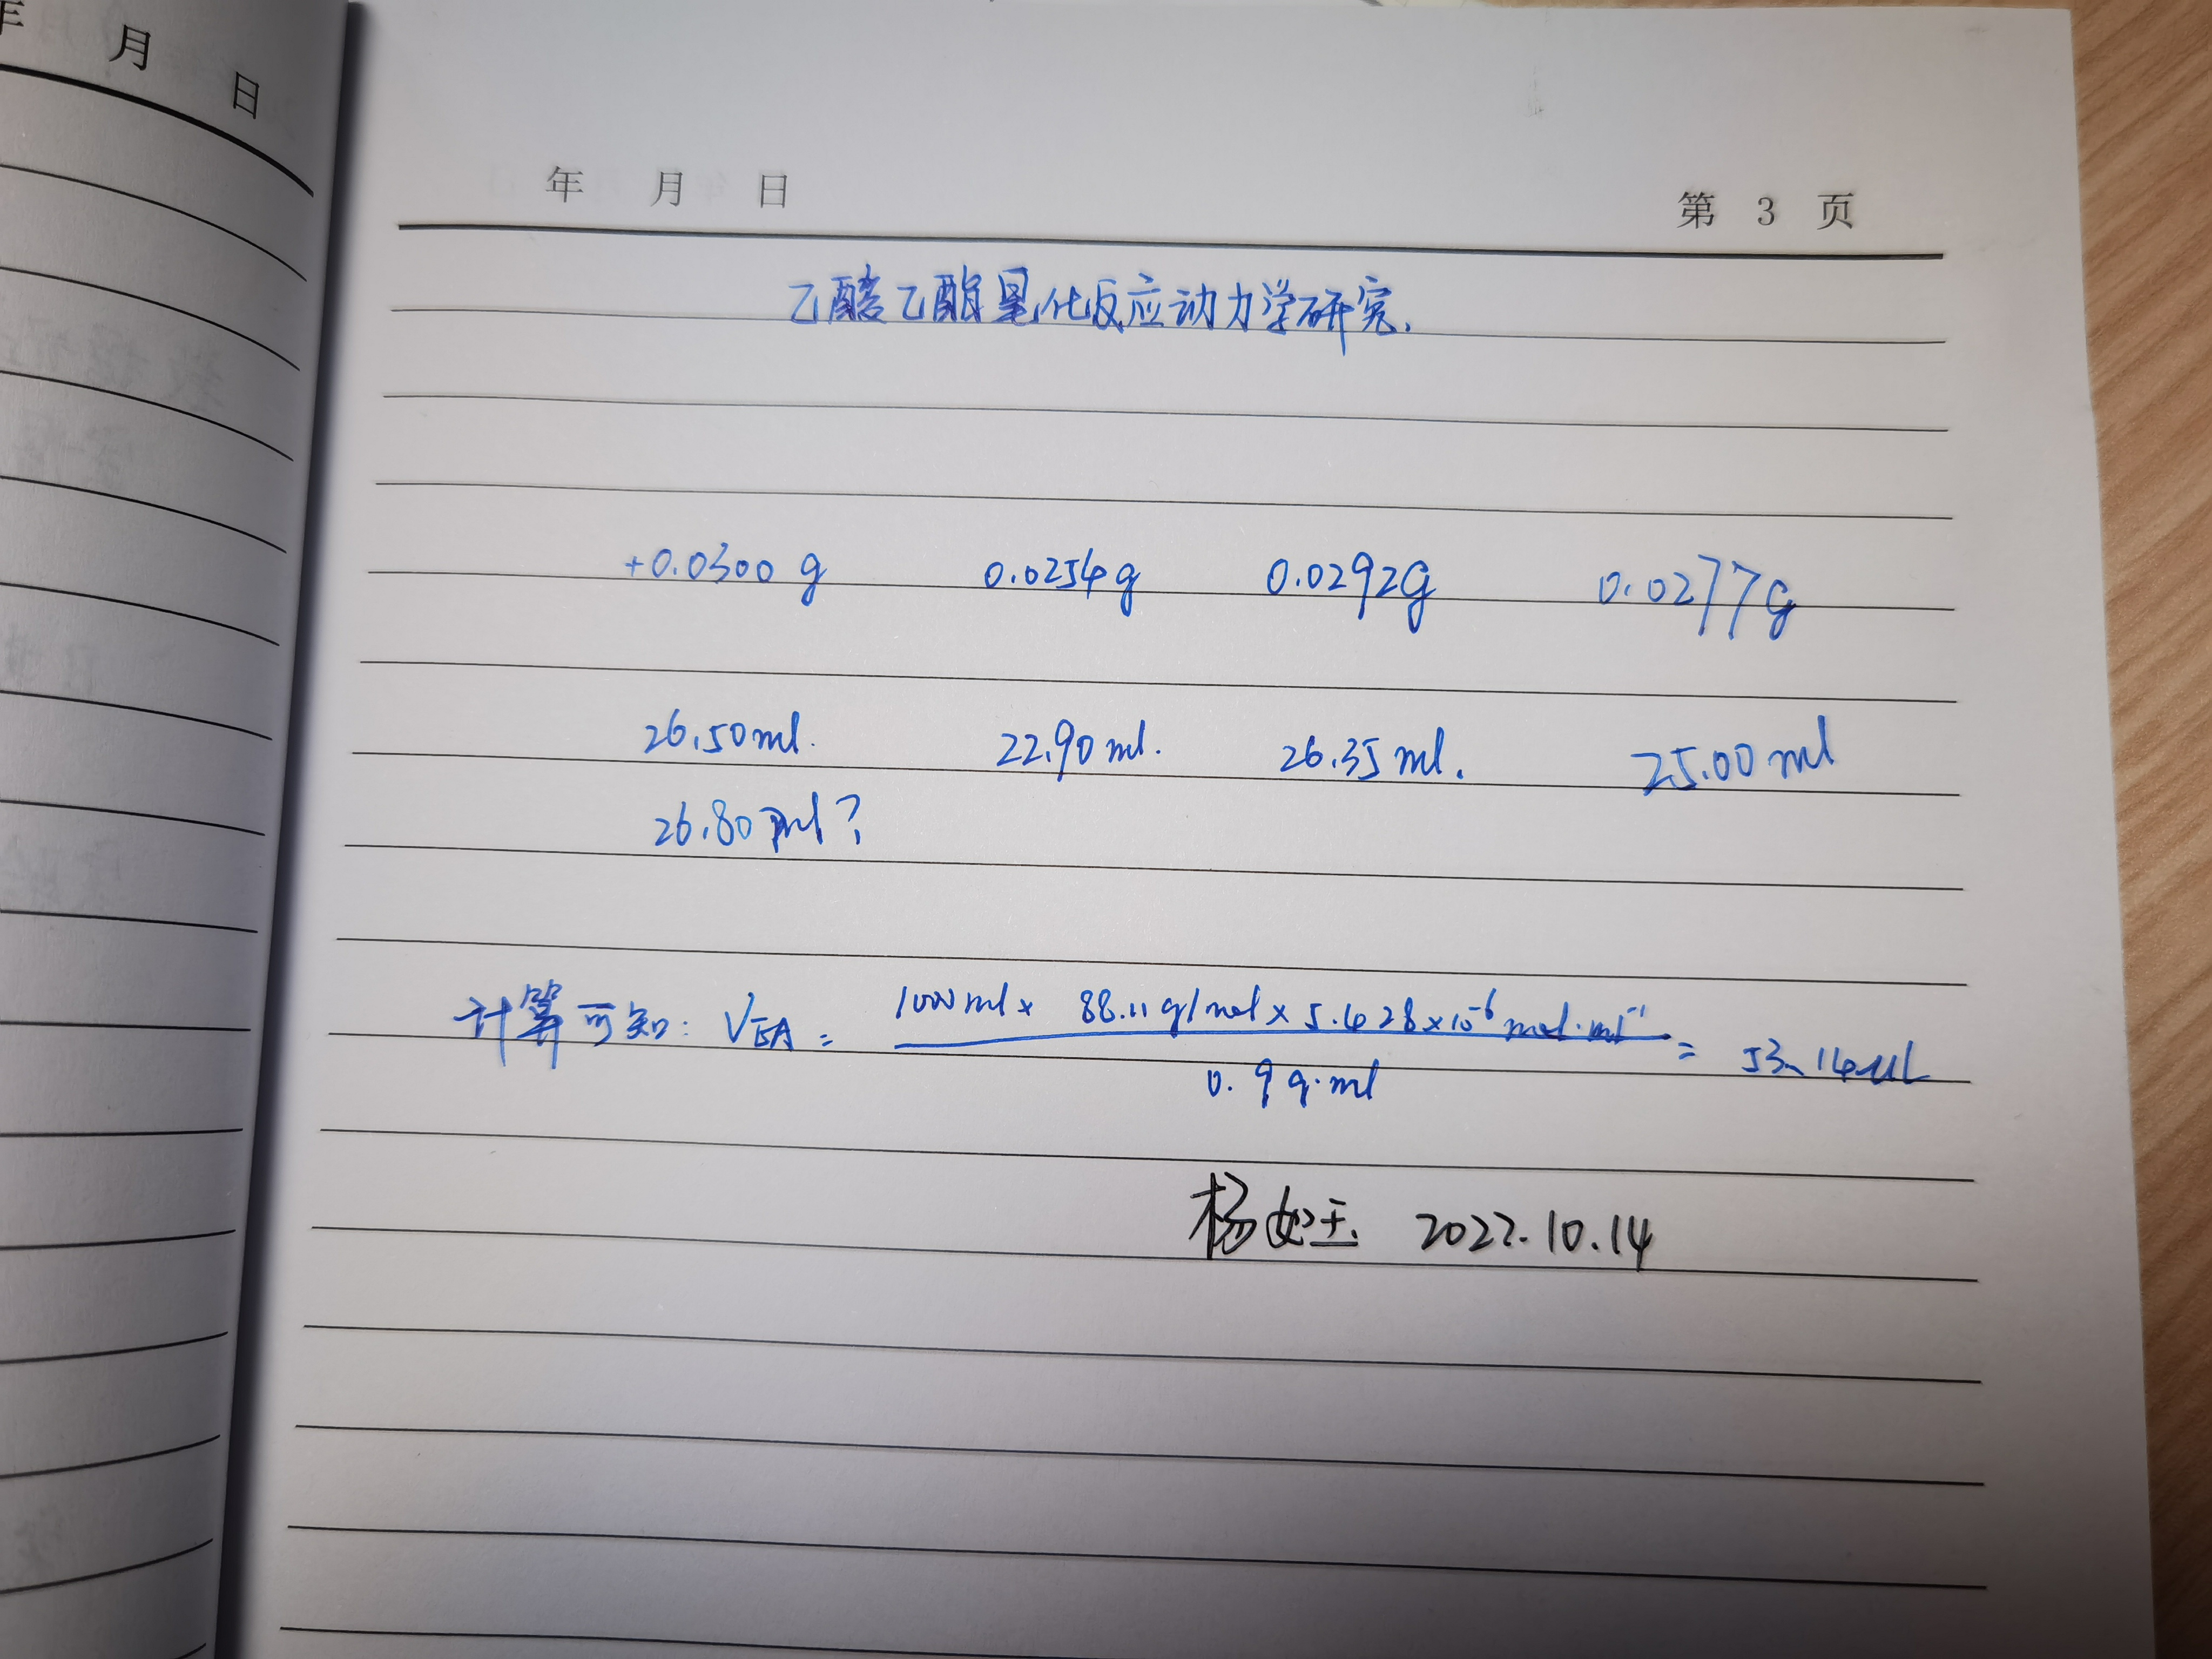
\includegraphics[width=0.8\textwidth]{原始数据.jpg}
    \caption{滴定数据记录}
    \label{fig}
\end{figure}

\end{document}
